Details about kernel states

\par
\par
\par
\hypertarget{states_states_intro}{}\subsection{Intro}\label{states_states_intro}
A Kernel state machine is a behavior model of the kernel core. Each state defines what methods are allowed.\hypertarget{states_states_fsm}{}\subsection{e\-Solid R\-T Kernel states}\label{states_states_fsm}
The kernel can be in one of the following states\-: \begin{center}

\begin{DoxyImageNoCaption}
  \mbox{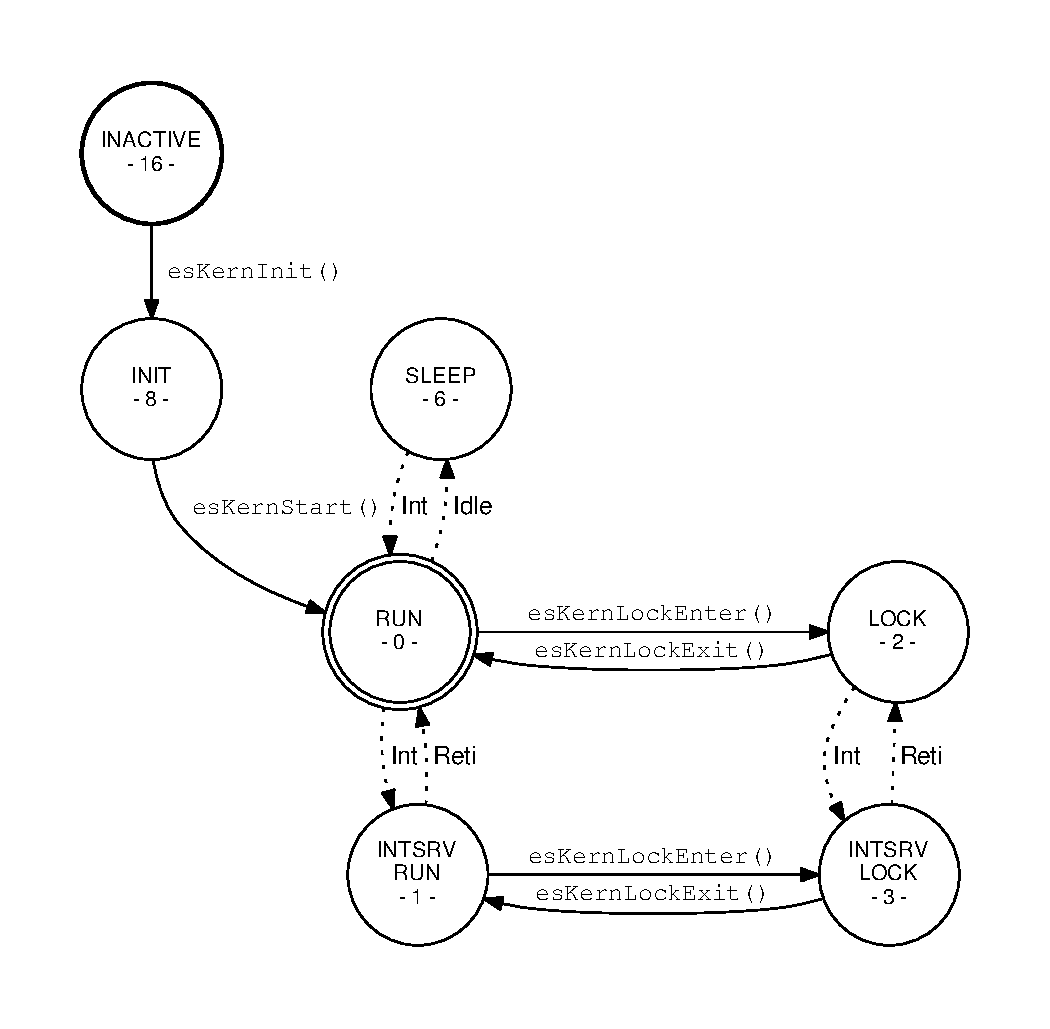
\includegraphics[width=\textwidth,height=\textheight/2,keepaspectratio=true]{dot_inline_dotgraph_1}}
\end{DoxyImageNoCaption}
\end{center}
 \begin{DoxyParagraph}{I\-N\-A\-C\-T\-I\-V\-E}
Inactive state of the kernel (Level 5). This state is entered after a physical reset. When the system is in this state all the maskable interrupt sources are disabled. In this state none of kernel internal data structures are initialized. In this state it is not possible to use any Kernel A\-P\-I except \hyperlink{group__kern__intf_ga9e9ff699d62d6035cd51121bb3140704}{es\-Kern\-Init()}.
\end{DoxyParagraph}
\begin{DoxyParagraph}{I\-N\-I\-T}
Initialization state of the kernel (Level 4). In this state all internal data structures are initialized but the kernel is still not running. In this stage new threads can be created by calling \hyperlink{group__kern__intf_gac91734f3ee867b519f59bf81cc7fde88}{es\-Thd\-Init()} function. Also, the application is allowed to use A\-P\-I which is used to create kernel structures like Thread Queues \hyperlink{structesThdQ}{es\-Thd\-Q}. All the maskable interrupt sources are D\-I\-S\-A\-B\-L\-E\-D.
\end{DoxyParagraph}
\begin{DoxyParagraph}{R\-U\-N}
Normal, running state of the kernel (Level 0). To start multi-\/threading just call the \hyperlink{group__kern__intf_ga0e7a0a6b9c02df58de0f98de0229a09d}{es\-Kern\-Start()} function. This function will switch the kernel into {\ttfamily R\-U\-N} state and multi-\/threading of created threads will commence. During the {\ttfamily R\-U\-N} state you are allowed to create other task as well. All the interrupt sources are enabled and the system A\-P\-Is are accessible, threads are running. All the maskable interrupt sources are E\-N\-A\-B\-L\-E\-D.
\end{DoxyParagraph}
\begin{DoxyParagraph}{L\-O\-C\-K}
Scheduler locked state, no context switching (Level 2). The running state of the kernel can be switched to {\ttfamily L\-O\-C\-K} state where the scheduler is locked and no context switching is allowed. {\ttfamily L\-O\-C\-K} state is one way of preventing the access to a shared resource. One more reason to lock the scheduler would be during the accessing of special hardware (e.\-g. programming the F\-L\-A\-S\-H memory) which does not allow interruption of the running operation. Usage of scheduler locks should be kept at minimum. All the maskable interrupt sources are E\-N\-A\-B\-L\-E\-D.
\end{DoxyParagraph}
\begin{DoxyParagraph}{I\-N\-T\-S\-R\-V\-\_\-\-R\-U\-N or I\-N\-T\-S\-R\-V\-\_\-\-L\-O\-C\-K}
Interrupt Service state, no context switching (Levels 1 and 3). During the both states {\ttfamily R\-U\-N} and {\ttfamily L\-O\-C\-K}, an interrupt event can occur. When Interrupt Service Routine is executing the kernel is in {\ttfamily I\-N\-T\-S\-R\-V\-\_\-\-R\-U\-N} or {\ttfamily I\-N\-T\-S\-R\-V\-\_\-\-L\-O\-C\-K} state. Each state corresponds to the state where the execution was interrupted from and the kernel will return to it's original state.
\end{DoxyParagraph}
\begin{DoxyParagraph}{S\-L\-E\-E\-P}
When idle condition occurs the kernel will switch to {\ttfamily S\-L\-E\-E\-P} state (if power saving is enabled). In order to return to {\ttfamily R\-U\-N} state an interrupt must occur whether from system timer or any other interrupt source which must request a context switch upon exit from I\-S\-R.
\end{DoxyParagraph}
\begin{DoxyNote}{Note}
The level of state {\ttfamily I\-N\-A\-C\-T\-I\-V\-E} is the highest. As the kernel boots up the level is decremented. The running state is level 0. 
\end{DoxyNote}
